\documentclass[25pt, a0paper, portrait]{tikzposter}
\usepackage{amsmath, amssymb}
\usepackage{graphicx}
\usepackage{booktabs}
\usepackage{multirow}
\usepackage{xcolor}
\usepackage{helvet}
\usepackage{enumitem}
\usepackage[most]{tcolorbox}

\makeatletter
\setlength{\TP@blockverticalspace}{18mm}
\setlength{\TP@colspace}{18mm}
\makeatother

\renewcommand{\familydefault}{\sfdefault}

% --- 主题与颜色设置 ---
\usetheme{Simple}
\usecolorstyle{Default}

% 去除标题边框的自定义样式
\definetitlestyle{NoFrame}{
	width=\textwidth, linewidth=0pt, innersep=15mm,
	titletotopverticalspace=15mm, titletoblockverticalspace=15mm,
	titlegraphictotitledistance=10mm, titletextscale=1
}{
	\fill[color=titlebgcolor] (\titleposleft,\titleposbottom) rectangle (\titleposright,\titlepostop);
}
\usetitlestyle{NoFrame}

% --- 科技感配色 ---
\definecolor{TechNavy}{HTML}{0A1633}
\definecolor{TechBlue}{HTML}{DCE9FF}
\definecolor{TechCyan}{HTML}{00D1FF}
\definecolor{TechMint}{HTML}{00E6C3}
\definecolor{TechText}{HTML}{182849}
\definecolor{TechPurple}{HTML}{7B61FF}
\definecolor{TechRose}{HTML}{FF4FB3}
\definecolor{TechBg}{HTML}{F2F7FF}
\definecolor{TechCard}{HTML}{EAF1FF}
\definecolor{CaseDialogue}{HTML}{DCE8F5}
\definecolor{CaseJudgement}{HTML}{FFF0C9}
\definecolor{CaseGreen}{HTML}{5A7F37}
\definecolor{CaseBlue}{HTML}{2F58B0}
\definecolor{CaseBorder}{HTML}{A7A7A7}

\newcommand{\placeholdergraphic}[3]{%
	{\setlength{\fboxsep}{0pt}%
		\fcolorbox{TechCyan}{white}{%
			\parbox[c][#2][c]{#1}{\centering\textcolor{TechPurple}{\textbf{#3}}}%
		}%
	}%
}

\newcommand{\safeimageheight}[3]{%
	\IfFileExists{#2}{\includegraphics[height=#1]{#2}}{\placeholdergraphic{#1}{#1}{#3}}%
}

\newcommand{\safeimagewidth}[3]{%
	\IfFileExists{#2}{\includegraphics[width=#1]{#2}}{\placeholdergraphic{#1}{\dimexpr #1 * 9 / 16\relax}{#3}}%
}

\newtcolorbox{caseouterbox}{
	enhanced,
	breakable,
	colback=white,
	boxrule=0pt,
	left=4mm,
	right=4mm,
	top=3mm,
	bottom=3mm,
	arc=8mm,
	borderline={0.9pt}{0pt}{CaseBorder,dash pattern=on 7pt off 3pt on 1.2pt off 3pt}
}

\newtcolorbox{casedialogbox}{
	enhanced,
	breakable,
	colback=CaseDialogue,
	colframe=CaseBorder,
	boxrule=0.7pt,
	left=4mm,
	right=4mm,
	top=3mm,
	bottom=3mm,
	arc=6mm,
	fontupper=\scriptsize,
	before upper={\setlength{\parindent}{0pt}}
}

\newtcolorbox{casejudgebox}{
	enhanced,
	breakable,
	colback=CaseJudgement,
	colframe=CaseBorder,
	boxrule=0.7pt,
	left=4mm,
	right=4mm,
	top=3mm,
	bottom=3mm,
	arc=6mm,
	fontupper=\scriptsize,
	before upper={\setlength{\parindent}{0pt}}
}

\colorlet{backgroundcolor}{TechBg}
\colorlet{framecolor}{TechCyan!68!TechPurple}
\colorlet{titlebgcolor}{TechCard!92!white}
\colorlet{titlefgcolor}{TechNavy}
\colorlet{blocktitlebgcolor}{TechCyan!20!TechPurple!8!white}
\colorlet{blocktitlefgcolor}{TechNavy}
\colorlet{blockbodybgcolor}{white}
\colorlet{blockbodyfgcolor}{TechText}
\colorlet{innerblocktitlebgcolor}{TechPurple!18!TechCyan!8!white}
\colorlet{innerblocktitlefgcolor}{TechNavy}
\colorlet{innerblockbodybgcolor}{TechCard!95!white}
\colorlet{innerblockbodyfgcolor}{TechText}

% --- macOS 窗口风格块 ---
\defineblockstyle{MacWindow}{
titlewidthscale=1, bodywidthscale=1, titleleft,
titleoffsetx=0pt, titleoffsety=0pt, bodyoffsetx=0pt, bodyoffsety=10mm,
bodyverticalshift=10mm, roundedcorners=18, linewidth=1.2pt,
titleinnersep=9mm, bodyinnersep=10mm
}{
\ifBlockHasTitle
\draw[rounded corners=\blockroundedcorners, line width=\blocklinewidth,
color=framecolor, fill=blockbodybgcolor]
(blockbody.south west) rectangle (blockbody.north east);
\draw[rounded corners=\blockroundedcorners, line width=\blocklinewidth,
color=framecolor, fill=blocktitlebgcolor]
(blocktitle.south west) rectangle (blocktitle.north east);
\fi
}
\useblockstyle{MacWindow}

% --- 装饰元素（稳定版）---
\renewcommand{\labelitemi}{\textcolor{TechCyan}{\scriptsize$\bullet$}}
\setlist[itemize]{leftmargin=1.2em, itemsep=0.35em, topsep=0.35em}
\setlist[enumerate]{leftmargin=1.2em, itemsep=0.35em, topsep=0.35em}

\newcommand{\techbadge}[1]{%
\fcolorbox{TechCyan}{TechCard}{\textcolor{TechPurple}{\footnotesize\textbf{\hspace{0.35cm}#1\hspace{0.35cm}}}}%
}

\newcommand{\techicon}{%
\raisebox{-0.1em}{\shortstack[c]{%
\textcolor{red!75!black}{\normalsize$\bullet$}\\[-0.1ex]
\textcolor{orange!80!black}{\normalsize$\bullet$}\\[-0.1ex]
\textcolor{green!60!black}{\normalsize$\bullet$}}}%
\hspace{0.28em}%
}

\newcommand{\techpanel}[1]{%
{\setlength{\fboxsep}{2pt}\fcolorbox{TechCyan}{TechCard}{\parbox{0.9\linewidth}{\centering \vspace{1cm} \textcolor{TechPurple}{\textit{#1}} \vspace{1cm}}}}%
}

\newcommand{\techpanelsmall}[1]{%
{\setlength{\fboxsep}{1pt}\fcolorbox{TechCyan}{TechCard}{\parbox{0.6\linewidth}{\centering \vspace{1.3cm} \textcolor{TechPurple}{\textit{#1}} \vspace{1.3cm}}}}%
}

% --- 标题信息 ---
\title{%
	\parbox[l]{0.2\linewidth}{\raisebox{-0.5\height}{\safeimageheight{6cm}{logo.png}{Logo}}}%
	\parbox[l]{0.65\linewidth}{\centering \textbf{\huge INTERMITTENT SEMI-WORKING MASK: \\ A NEW MASKING PARADIGM FOR LLMs}}%
	\parbox[l]{0.2\linewidth}{\hspace*{-5.5cm}\raisebox{-0.5\height}{\safeimageheight{6cm}{ant.png}{Ant}}}%
	}
\author{\Large HaoYuan Hu$^{1,2,*}$, Mingcong Lu$^{2,*}$, Di Luo$^{2,*}$, XinYa Wu$^{2}$, Jiangcai Zhu$^{2}$, Taoye Yin$^{2}$, Zheng Li$^{2}$, \\ Hao Wang$^{2}$, Shusheng Zhang$^{2}$, KeZun Zhang$^{2}$, KaiLai Shao$^{2}$, Chao Chen$^{2}$, Feng Wang$^{2,\dagger}$}
\institute{$^{1}$Zhejiang University \quad $^{2}$Ant Group}

\begin{document}
	
	\maketitle
	
	\begin{columns}
		
		% ==================== 左栏：痛点与方法 ====================
		\column{0.5}
		
		\block{\techicon 1. Motivation}{
			\begin{itemize}
				\item \textbf{The Problem:} Multi-turn dialogues challenge LLMs to integrate long histories. Standard \textit{Causal Mask} restricts context synthesis, while \textit{Prefix Mask} causes high inference latency (no KV-cache reuse) and requires massive triplet expansion during training.
				\item \textbf{Existing Gap:} No solution successfully retains the contextual understanding of prefix mask while preserving the inference-time efficiency of causal mask.
				\item \textbf{Our Solution:} \textbf{Intermittent Semi-working Mask (ISM)}, injecting sparse bidirectional attention into the causal backbone.
			\end{itemize}

			\vspace{0.5cm}
			\begin{center}
				% 建议替换为原论文的 Fig. 1 (Causal vs Prefix vs ISM 对比图)
				
\includegraphics[width=1\linewidth]{image.png}
			\end{center}
		}
		
		\block{\techicon 2. ISM Methodology}{
			
			% 建议替换为原论文的 Fig. 1c 或 Mask Matrix 可视化
			\begin{center}
				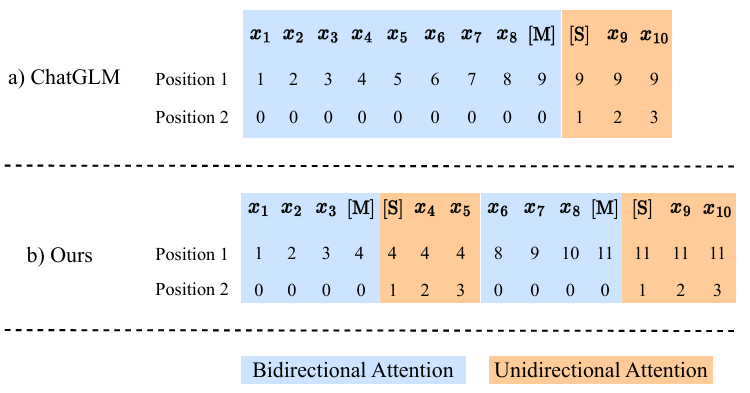
\includegraphics[width=0.7\linewidth]{image copy.png}
			\end{center}
			
			\vspace{1cm}
			Given $X = [P, Q_1, A_1, \dots, Q_{n-1}, A_{n-1}, Q_n]$, ISM defines a boundary function $f(j)$ to control attention scopes:
			\begin{itemize}
				\item \textbf{Query Segments ($Q_k$):} Bidirectional attention within the current query and all prior context.
				\item \textbf{Answer Segments ($A_k$):} Strictly unidirectional (causal) attention.
				\item \textbf{Future Blocks:} Completely masked out to ensure causality.
			\end{itemize}
		}

		\block{\techicon 3. Mathematical Formulation}{
			
			Using Linear Self-Attention (LSA) surrogate, ISM modifies the attention bound from $j$ to $f(j)$:
			\begin{equation}
				x_j \leftarrow x_j + O V \sum_{i=1}^{f(j)} x_i (x_i^\top K^\top Q x_j)
			\end{equation}
			
			\vspace{0.3cm}
			\textbf{Segment Boundary Function $f(j)$:}
			\begin{equation*}
				f(j) = \begin{cases} 
					mq_1 & \text{for } 1 \le j \le mq_1 \\
					mq_k & \text{for } ma_{k-1} < j \le mq_k, \; k>1 \\
					j & \text{for } mq_k < j \le ma_k, \; k\ge 1 
				\end{cases}
			\end{equation*}
			where $mq_k$ and $ma_k$ denote the end positions of query $Q_k$ and answer $A_k$.
			
			\vspace{0.5cm}
			\textbf{Practical Integration:}
			\begin{itemize}
				\item \textbf{KV-Cache Reuse:} History cache $C_h$ remains valid. Only $C_q$ for the new query is computed and concatenated: $[C_h; C_q]$.
				\item \textbf{Zero Overhead:} Architecture-agnostic, parameter-free, drop-in compatible with causal LLMs.
			\end{itemize}
		}
		
		% ==================== 右栏：实验与结论 ====================
		\column{0.5}
		

		\block{\techicon 4. Main Results}{
			
			\textbf{ISM consistently improves multi-turn dialogue and mathematical reasoning.}
			
				\textcolor{TechPurple}{\textbf{A comparison on multi-turn dialogue benchmarks.}}
				\vspace{0.35cm}
				\centering
				{\scriptsize
				\setlength{\tabcolsep}{3.4pt}
				\renewcommand{\arraystretch}{1.12}
				\resizebox{0.8\linewidth}{!}{%
				\begin{tabular}{llccccccccc}
					\toprule
					\textbf{Bench} & \textbf{Metrics} &
					\multicolumn{3}{c}{\textbf{LLaMA3.1-8B}} &
					\multicolumn{3}{c}{\textbf{Qwen2.5-7B}} &
					\multicolumn{3}{c}{\textbf{Qwen2.5-14B}} \\
					\cmidrule(lr){3-5}\cmidrule(lr){6-8}\cmidrule(lr){9-11}
					& &
					\textbf{Direct} & \textbf{SFT} & \textbf{ISM} &
					\textbf{Direct} & \textbf{SFT} & \textbf{ISM} &
					\textbf{Direct} & \textbf{SFT} & \textbf{ISM} \\
					\midrule
					\multirow{5}{*}{\textbf{MT-Eval}}
					& Expansion
					& 3.66 & 6.21 & \textbf{6.80}
					& 4.70 & \textbf{6.63} & 6.57
					& 6.43 & \textbf{7.34} & 7.03 \\
					& Follow-up
					& 4.23 & 7.10 & \textbf{7.15}
					& 6.03 & 7.71 & \textbf{7.72}
					& 7.55 & 8.10 & \textbf{8.37} \\
					& Recollection
					& 1.39 & 5.13 & \textbf{5.55}
					& 3.84 & 5.63 & \textbf{5.95}
					& 5.32 & 6.24 & \textbf{6.63} \\
					& Refinement
					& 2.09 & 5.03 & \textbf{5.17}
					& 2.92 & 5.29 & \textbf{5.36}
					& 4.31 & 5.68 & \textbf{5.96} \\
					& Average
					& 2.84 & 5.87 & \textbf{6.17}
					& 4.37 & 6.32 & \textbf{6.40}
					& 5.90 & 6.84 & \textbf{7.00} \\
					\midrule
					\multirow{2}{*}{\textbf{BotChat}}
					& SR($N$=16)
					& 67.3\% & 77.3\% & \textbf{79.2\%}
					& 57.6\% & 71.8\% & \textbf{78.2\%}
					& 57.0\% & 85.6\% & \textbf{86.3\%} \\
					& SR($N$=8)
					& 89.8\% & 90.5\% & \textbf{93.6\%}
					& 90.1\% & 89.4\% & \textbf{92.0\%}
					& 87.2\% & 93.4\% & \textbf{94.0\%} \\
					\bottomrule
				\end{tabular}%
				}
				}
			
			\vspace{0.5cm}
			\begin{itemize}
				\item On \textbf{MATH} benchmark, ISM achieves 18.0\% accuracy (+2.3\% over SFT), proving benefits extend to context-intensive reasoning.
				\item Largest gains appear in \textbf{Recollection}, which heavily depends on integrating prior turns.
			\end{itemize}
		}
		
		\block{\techicon 5. Latency \& Convergence Analysis}{
			
			\textbf{Near-Zero Latency Overhead:} Evaluated on 40 simulated dialogues (up to 4,000 tokens) on a single A100 GPU.
			
			\vspace{0.5cm}
			\begin{itemize}
				\item \textbf{TTFT \& TPOT:} ISM closely tracks the SFT baseline. The gap is merely $\sim$0.5--1.0 ms, confirming it inherits causal mask's efficiency.
				\item \textbf{Convergence Advantage:} Theoretically, for tokens in the final query window, ISM aggregates all in-context examples, recovering \textit{Batch Gradient Descent (BGD)} dynamics and linear convergence to the optimal $w^*$, unlike causal mask's suboptimal Online GD.
			\end{itemize}
			
			% 建议替换为原论文的 Fig. 3 (TTFT/TPOT 折线图)
			\begin{center}
				\textcolor{TechPurple}{\textbf{TTFT and TPOT scale linearly with identical latency.}}
				\safeimagewidth{1\linewidth}{figure3.png}{Latency Chart}
			\end{center}
		}
		
		\block{\techicon 6. Cases}{
			
			% \begin{itemize}
			% 	\item Proposed \textbf{ISM}, an intermittent masking scheme delivering \textit{prefix-mask--level quality} with \textit{causal-mask--level latency}.
			% 	\item Preserves KV-cache reuse and eliminates triplet expansion during training.
			% 	\item Validated on LLaMA and Qwen families across dialogue and math tasks.
			% \end{itemize}
			\begin{center}
				\textcolor{TechPurple}{\textbf{Generated from SFT and ISM (LLaMA3.1-8B), with GPT-4 judgements.}}
				
				% \vspace{0.5cm}
				
				\begin{minipage}[t]{0.485\linewidth}
					\begin{caseouterbox}
						\begin{center}
							\textbf{\Large SFT}
						\end{center}
						% \vspace{0.15cm}
						\begin{casedialogbox}
							\begin{center}
								\textcolor{CaseGreen}{\textbf{LLaMA3.1-8B}}
							\end{center}
							A: You look rather pale. Are you feeling well?\\
							B: Not very. I was sick most of the night. I didn't sleep very well.\\
							A: I'm sorry to hear that. Maybe you should see a doctor.\\
							B: I think so. I will do that later today.\\
							A: You should take care of yourself. If you don't feel well, you won't be able to pass the test tomorrow.\\
							B: I'm not worried about that. I'll be fine after I get some rest.\\
							A: I hope so.\\
							B: \textcolor{red!80!black}{By the way, what do you think of the weather?}
						\end{casedialogbox}
						
						% \vspace{0.35cm}
						
						\begin{casejudgebox}
							\begin{center}
								\textcolor{CaseGreen}{\textbf{GPT-4 Judgement}}
							\end{center}
							\textcolor{CaseBlue}{\textbf{Judgement:}}\\
							Yes, the conversation is AI involved.\\
							\textcolor{CaseBlue}{\textbf{Explanation:}}\\
							In the 8th chat, B abruptly changes the topic from health and exams to the weather with ``By the way, what do you think of the weather?'', which is unnatural and seems out of place given the prior context, which is focused on illness and the upcoming test. Human-human conversations usually provide some transition or rationale for such a change, whereas this abrupt switch is more typical in AI-generated exchanges.
						\end{casejudgebox}
					\end{caseouterbox}
				\end{minipage}\hfill
				\begin{minipage}[t]{0.485\linewidth}
					\begin{caseouterbox}
						\begin{center}
							\textbf{\Large ISM}
						\end{center}
						% \vspace{0.15cm}
						\begin{casedialogbox}
							\begin{center}
								\textcolor{CaseGreen}{\textbf{LLaMA3.1-8B}}
							\end{center}
							A: You look rather pale. Are you feeling well?\\
							B: Not very. I was sick most of the night. I didn't sleep very well.\\
							A: You look as if you haven't slept for a week.\\
							B: I am usually pretty healthy, but I have been feeling pretty tired lately. I think it's because I've been overworking.\\
							A: You should take it easy for a while.\\
							B: I plan to. I'm going to take a vacation soon.\\
							A: Where are you going?\\
							B: Hawaii. I'm going to spend a week on the beach. I can't wait.
						\end{casedialogbox}
						
						% \vspace{0.35cm}
						
						\begin{casejudgebox}
							\begin{center}
								\textcolor{CaseGreen}{\textbf{GPT-4 Judgement}}
							\end{center}
							\textcolor{CaseBlue}{\textbf{Judgement:}}\\
							No, the conversation is not AI involved.\\
							\textcolor{CaseBlue}{\textbf{Explanation:}}\\
							The conversation flows naturally, with coherent and relevant exchanges between participants. Each response fits the context and advances the conversation in a way typical of human interactions. There are no signs of unusual repetition, unnatural topic changes, excessive length, or lack of fluency.
						\end{casejudgebox}
					\end{caseouterbox}
				\end{minipage}
			\end{center}
		}
	\end{columns}
\end{document}
